\documentclass[oneside,final,14pt,a4paper]{extreport}



\usepackage[utf8]{inputenc}
%\usepackage[english, russian]{babel}
\usepackage[russianb]{babel} % адаптация русского языка
\usepackage{vmargin} % настройка размера полосы набора
\setpapersize{A4}
\setmarginsrb{2cm}{2cm}{2cm}{2cm}{0pt}{0mm}{0pt}{13mm} % {левое поле}{верхнее поле}{правое поле}{нижнее поле}{колонтитулы}{колонтитулы}{колонтитулы}{номер страницы}
\usepackage{indentfirst} % отделять первую строку раздела абзацным отступом
\usepackage{graphicx} % подключение библиотеки для работы с внешними картинками
\usepackage{setspace} % для изменения межстрочного интервала
\sloppy % выравнивание текста
%\linespread{1.3} % полуторный интервал

\setstretch{1.5} % устанавливаем межстрочный интервал

\usepackage {titlesec}
% меняем заголовок для команды \chapter и запрещаем переносы слов
\titleformat{\chapter}{\hyphenpenalty=10000\normalfont\huge\bfseries\flushleft}{\thechapter\space\space}{0pt}{\huge}


%\usepackage[OT1]{fontenc}
%\usepackage{amsmath}
%\usepackage{amsfonts}
%\usepackage{amssymb}
%\usepackage{graphicx}
%\usepackage[left=2cm,right=2cm,top=2cm,bottom=2cm]{geometry}
%\usepackage{cmap} % для кодировки шрифтов в pdf
% \usepackage{indentfirst} % отделять первую строку раздела абзацным отступом


\makeatletter
\renewcommand{\@biblabel}[1]{#1\space} % Заменяем библиографию с [number] на просто number:
\makeatother


\begin{document}





% ТИТУЛЬНЫЙ ЛИСТ НАЧИНАЕТСЯ
\thispagestyle{empty}
\begin{titlepage}

\begin{figure}
	\centering
	
\includegraphics[width=0.5\textwidth]{logo.eps}\\
\end{figure}

\begin{spacing}{1.0} % устанавливаем межстрочный интервал
\begin{center} % центрируем текст
	{\small
		Московский государственный университет имени М.В. Ломоносова \\
		Факультет вычислительной математики и кибернетики \\
		Кафедра автоматизации систем вычислительных комплексов \\
	}
	\vspace{4cm}
	{\large Романов Андрей Романович \\}
	\vspace{1cm}
	{\large\bfseries
		Разработка системы обеспечения надежного и \\
		масштабируемого 	виртуального сетевого сервиса в \\
		облачной среде \\
	}
	\vspace{1cm}
	ВЫПУСКНАЯ КВАЛИФИКАЦИОННАЯ  РАБОТА
\end{center}
\vfill
\begin{flushright}
\begin{small}
	{\bfseries Научный руководитель: \\}
	к.ф.-м.н. \\
	В.А. Антоненко \\
\end{small}
\end{flushright}

\vfill

\centerline{Москва, 2016}
\end{spacing}
\end{titlepage}
% ТИТУЛЬНЫЙ ЛИСТ ЗАКАНЧИВАЕТСЯ
\setcounter{page}{2}





\chapter*{Аннотация}
В данной работе рассматриваются проблемы организации надежной работы и масштабируемости виртуального сетевого сервиса (Virtual Network Service, VNS). Рассмотрены существующие решения организации работы виртуальных сетевых функций (Virtual Netrowk Function, VNF).

В рамках выпускной квалификационной работы разработан программный комплекс, позволяющий в автоматическом режиме обеспечивать отказоустойчивость и масштабируемость виртуальных сетевых функций в облаке.





% Оглавление
\tableofcontents % генерация оглавления





\chapter*{Введение}
\addcontentsline{toc}{chapter}{Введение} % добавить Введение в оглавление

В современных сетях функционирует огромное количество сервисов: маршрутизация (routing), трансляция сетевых адресов (NAT), сетевой экран (firewall), туннелирование (VPN), проски-сервер и т.д.. Многие из них реализованы в одном устройстве. Для эффективной работы сервисов нагрузку распределяют сразу на несколько таких устройств. При необходимости в новой фукнции требуется купить новое оборудование, которое будет обладать прочими ненужными функциями. При высокой нагрузке, устройство не будет справляться со своими задачами, а значит придется купить еще одно. В случае недостаточной нагрузки устройства будут простаивать. Здесь возникает проблема динамической масштабируемости сервиса в зависимости от его загрузки. Известно, что при наличии нескольких схожих по функциональности устройств от разных произодителей, могут возникать конфликты в их работе. Таким образом, одним из решений является приобретение оборудование только от одного вендора. Со временем производитель отказывается поддерживать устаревшее оборудование. И в этом случае остается крайний вариант - приобретение новых устройств взамен устаревших.

Таким образом можно выделить ключевые проблемы организации работы сетевого сервиса:
\begin{itemize}
	\item приобретение оборудования с избыточной функциональностью;
	\item требуется рассчитывать производительность сервиса исходя из максимальной возможной нагрузки;
	\item простаивание оборудования в случае, если нагрузка не является пиковой;
	\item зависимость от производителя оборудования (тех. обслуживание, устаревание оборудования, невозможность модифицировать сервис без вмешательства производителя);
\end{itemize}

Концепция виртульных сетевых функций (Network Function Virtualization, NFV) --- это молодая технология, позволяющая виртуализировать некоторые программные сервисы, которые на данный момент реализованы лишь на физических устройствах. NFV работает в рамках модели SaaS (Software as a Service, программное обеспечение как услугу) и обладает такими качествами, как:
\begin{itemize}
	\item масштабируемость - в зависимости от загруженности сервиса будет работать тот объем инфраструктуры, который необходим для надежной работы;
	\item надежность - в случае сбоев в работе сервиса будут предприниматься действия по восстановлению его работы в автоматическом режиме;
	\item гибкость - виртуализация позволяет быстро развертывать сервисы на новой инфраструктуре;
	\item безопасность - данные клиентов защищены, так как программные сервисы работают изолированно друг от друга.
\end{itemize}

Организация ETSI разработала высокоуровневую архитектуру ETSI NFV Management and Orchestration (ETSI NFV MANO). Главной особенностью архитектуры является оптимальное использование инфраструктуры: она выделяется для каждой функции по запросу в необходимом количестве. Базовыми блоками, из которых строятся виртуальные сетевые сервисы, являются виртуальные сетевые функции (VNF). Платформа на базе ETSI NFV MANO умеет размещать VNF на подконтрольной инфраструктуре. В результате комбинирования блоков VNF получаются виртуальные сетевые сервисы (VNS), которыми пользуются клиенты платформы.





\chapter{Постановка задачи}
Разработать решение, управляющее жизненным циклом виртуальных сетевых сервисов, обеспечивающее их надежную работу и масштабируемость.

Решение должно удовлетворять следующим требованиям:
\begin{itemize}
	\item по запросу осуществлять подписку и отписку пользователей от виртуальных сетевых сервисов в рамках модели Software as a Service (SaaS);
	\item при возникновении неисправности принимать меры по восстановлению корректной работы сервиса в автоматическом режиме (healing);
	\item обеспечивать масштабируемость инфраструктуры сервиса в автоматическом режиме (scaling);
	\item решение должно быть независимым от платформы виртуализации инфраструктуры;
	\item решение должно быть согласовано с высокоуровневой архитектуры ETSI NFV MANO;
	\item поддержка нескольких плафторм виртуализации инфраструктуры одновременно;
\end{itemize}





\chapter{Обзор предметной области}
\section{Общее описание NFV}
В 2004 году была предложена идея организации сетевой инфраструктуры с целью снижения затрат и ускорения внедрения новых услуг. Она состояла в объединении ядра сети и сети доступа в единую платформу. Однако без виртуализации идея не получила широкого распространения.\cite{nfv-state2}.

NFV предполагает использование виртуализированной инфраструктуры для функционирования услуг. Концепция предлагает использование технологий для виртуализации функций в виде составных элементов, которые могут быть связаны для создание телекоммуникационных сервисов. 

Таким образом, виртуальная сетевая функция (VNF) --- это описание требуемой инфраструктуры, требуемого программного обеспечения, параметров подключения пользователей к это услуге и т.д.. Заметим, что программное обеспечение, описанное в VNF должно иметь ограниченную и законченную функциональность. Не следует виртуализировать сложное программное обеспечение, так как оно будет использовать дополнительные ресурсы инраструктуры.

Виртуальный сетевой сервис (VNS) - это некоторое множество связанных между собой виртуальных сетевых функций. Это конечная услуга, которая будет предоставляться клиентам. Концепция предполагает внутреннее представление VNS как произвольное непустое множество, состоящее из VNF. При этом VNF как-то связаны друг с другом.

По мнению автора, наиболее интересен случай цепочек виртуальных сетевых функций (VNF chaining). В этом случае можно считать каждую VNS как цепочку сетевых функций. Близкую аналогию можно провести с математическим понятием функции. Пусть 'x' - это входящий трафик некоторого объема. Тогда результатом работы сервиса S, состоящего из последовательной цепочки функций f1, f2, f3 будет трафик y, такой что:

% TODO сделать формулой
y = f3(f2(f1(x))) = S(x)

В результате трафик 'x' трансформировался в трафик 'y'. S - это суперпозиция функций f1, f2, f3.


\section{Архитектура ETSI NFV MANO}
Европейский Институт Телекоммуникационных Стандартов (ETSI) в 2013 году опубликовал высокоуровневые рекомендации по разработке платформы, управляющий виртуальными сетевыми сервисами Network Function Virtualization Management and Orchestration (NFV MANO). Основные цели документы - стандартизировать интерфейсы каждого модуля в платформе.\cite{nfv-mano-state1} Как показано на Рис.~\ref{nfv-mano-image1}, в NFV MANO имеется 3 основных модуля:

\begin{enumerate}
	\item менеджер виртуальной инфраструктуры (Virtualized Infrastructure Manager, VIM)
	\item менеджер виртуальных сетевых функций (Virtual Network Function Manager, VNFM)
	\item оркестратор виртуальных сетевых сервисов (Network Function Virtualization, NFVO)
\end{enumerate}

\begin{figure}[h]
\center{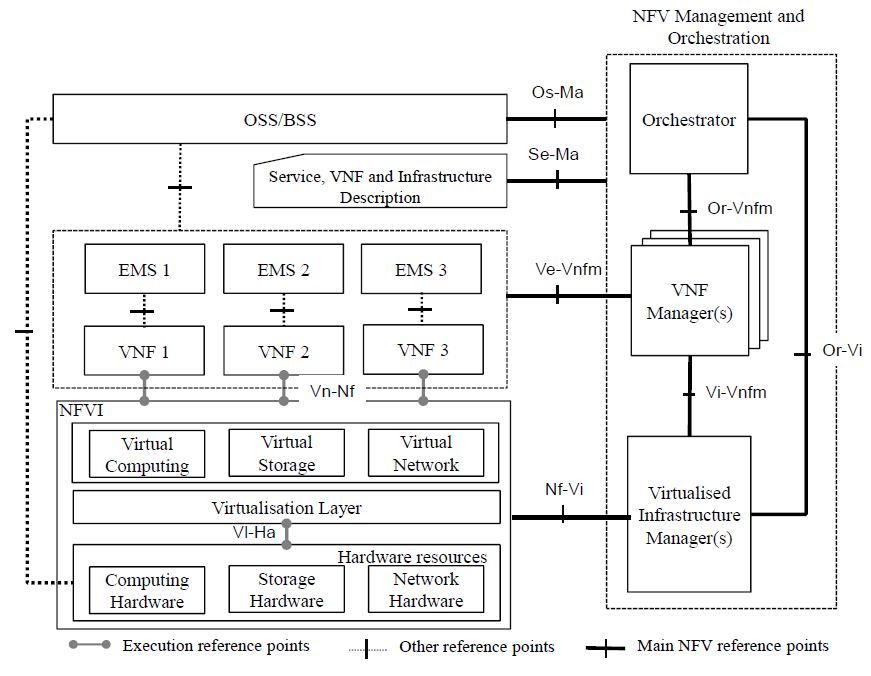
\includegraphics[width=0.95\textwidth]{nfv-mano}}
\caption{Архитектура NFV Management and Orchestration}
\label{nfv-mano-image1}
\end{figure}

Каждый модуль обеспечивает свой слой виртуализации. VIM занимается виртуализацией физических ресурсов. Менеджер функций предоставляет набор функций, размещенных на виртуальных ресурсах. Оркестратор управляет сетевыми сервисами, построенными на базе виртуальных сетевых функций.

Так же в архитектуре присутствуют неосновные модули:
\begin{itemize}
	\item описание виртуальных сетевых сервисов, функций и используемой ими инфраструктуры. В NFV MANO блоки, которые содержат такие описания, называют каталогами (catalog). В платформах, разрабатываемых на базе NFV MANO, обычно функции каталогов выполняет менеджеры соответствующего уровня (оркестратор сервисов, менеджер функций, VIM);
	\item система управления элементами (Element Management System, EMS). Система управляет работой элементов экземпляра виртуальной сетевой функции, отвечает за параметры функции. Данная система взаимодействует с менеджером функций через закрытые интерфейсы. Поэтому в существующих решениях, известных автору, данный модуль включен в состав менеджера функций.
\end{itemize}

Далее рассмотрим подробнее основные модули NFV MANO.

\subsection{Менеджер виртуальной инфраструктуры}
Менеджер инфраструктуры обеспечивает виртуализацию физической инрафструктуры в рамках одного домена. NFV MANO предполагает использование нескольких менеджеров инфраструктуры в одном домене. В задачи модуля входит:

\begin{itemize}
	\item управление полным жизненным циклом виртуальных ресурсов в рамках одного домена
	\begin{itemize}
		\item управление вычислительными ресурсами (computing resource) и хранилищами (storage);
		\item управление сетевыми ресурсами (networking resource), то есть управление коммутаторами, роутерами, сетевая настройка;
		\item остальные задачи гипервизора (асбтракция физической инфраструктуры, эффективное отображение ресурсов на их виртуальные аналоги и т.д.);
	\end{itemize}
	\item иметь полную информацию о доступных физических ресурсах и о запущенной виртуальной инфраструктуре;
	\item мониторинг за состоянием виртуальных ресурсов, обнаружение отказов оборудования, виртуальных машин, програмного обеспечения;
	\item оповещать остальные модули о смене состояния виртуальной инфраструктуры;
	\item предоставление интерфейса для использования виртуальной инфраструктуры и для мониторинга физической инфраструктуры.
\end{itemize}

Подробнее о функциях VIM, и его спецификациях можно прочитать в стандарте \cite{nfv-mano-official-2016-04}.

\subsection{Менеджер виртуальных сетевых функций}
Менеджер виртуальных сетевых функций (VNFM) --- это основной модуль архитектуры NFV MANO, ответственный за  полный жизненный цикл виртуальных сетевых функций. Архитектура предполагает возможность наличие нескольких менеджеров функций. Однако на момент написания работы остается неясным, необходимо ли наличие нескольких модулей.

В NFV MANO следует отличать два понятия: описание виртуальной сетевой функции (VNF description) и экземпляр виртуальной сетевой функции (VNF instance). Когда говорят про сетевую функцию, чаще всего имеют ввиду ее спецификации, то есть ее описание. Экземпляр VNF - это виртуальная инфраструктура, которая уже размещена поверх физической, и полностью удовлетворяют своему описанию (спецификациям). Таким образом, для каждой VNF существует единственное описание и множество ее экземпляров. Все экземпляры функции независимы друг от друга. В общем случае, они могут быть размещены в разных доменах (в разных VIM).

В задачи модуля входит:

\begin{itemize}
	\item регистрация и удаление VNF(в случае, если менеджер функций управляет сразу несколькими функциями);
	\item владение полной информации о всех спецификациях функции
	\begin{itemize}
		\item топология инфраструктуры, которую необходимо разместить для работы функции;
		\item входные параметры функции (TODO: привести пример);
		\item исчерпывающая информация о программном обеспечении виртуальных машин;
		\item описание событий, по которым можно судить о состоянии функции (например, в ситуации, когда инфраструктура экземпляра функции недоступна, можно считать, что функция не работает)
		\item описание триггеров на вышеуказанные события (перезапустить виртуальную машину в случае, если она не отвечает на команду ping в течении 5 секунд)
	\end{itemize}
	\item управление жизненным циклом виртуальной функции
	\item отслеживание неисправностей в работе программного обеспечения функции;
	\item реагировать на неисправности в работе VNF в соответствии с ее описанием (применить горизонтальное масштабирование в ответ на событие о недостатке производительности виртуальной машины);
	\item после размещения виртуальной инфраструктуры инициализировать ее, установить и настроить все необходимое для работы функции программное обеспечение;
	\item обновление программного обеспечения уже размещенных виртуальных функций;
	\item оповещать остальные модули о событиях, связанных с работой VNF;
\end{itemize}

Более подробную спецификацию менеджера виртуальных функций можно прочитать в стандарте \cite{nfv-mano-official-2016-04}.

\subsection{Оркестратор виртуальных сетевых сервисов}
Оркестратор сетевых сервисов решает две основные задачи:
\begin{itemize}
	\item оркестрация ресурсов между несколькими менеджерами инфраструктуры, резервация ресурсов;
	\item управление жизненным циклом виртуальных сетевых сервисов;
\end{itemize}

Задача управления виртуальными сервисами нетривиальна. Она включает в себя множество подзадач:

\begin{itemize}
	\item предоставление интерфейса создания, удаления, изменения, обновления VNS;
	\item авторизация для управления сетевыми сервисами, разграничение прав доступа;
	\item синхронизация работы с менеджерами функций;
	\item отслеживание неисправностей в работе сервисов;
	\item реакция на события, связанные с изменением состояния сервиса;
	\item оповещение остальных модулей об изменении состояния сервисов;
	\item резервация ресурсов под сервисы с помощью модуля VIM;
\end{itemize}

Более конкретный стандарт архитектуры NFV оркестратора находится в разработке, поэтому информацию о менеджере виртуальных сетевых сервисов можно получить, например, в высокоуровнем стандарте \cite{nfv-mano-official-2016-04}.





\chapter{Обзор существующиз NFV платформ}
\section{Open Platform for NFV}
Open Platform for NFV (OPNFV) - это платформа с открытым исходным кодом, на базе которой можно создавать компоненты  идеологии NFV. Проект OPNFV, используя архитектуру ETSI NFV MANO, фокусируется на разработке менеджера инфраструктуры (NFVI) архитектуры NFV MANO.\cite{opnfv-official}
Основные цели проекта:
\begin{itemize}
	\item разработка интегрированной и протестированной открытой платформы, которая сможет быть использована для построения NFV, ускорения внедрения новых продуктов и сервисов;
	\item привлечение заинтересованных лиц со стороны конечных заказчиков для удовлетворения требований пользовательского сообщества.
	\item создать экосистему NFV решений, основанную на открытых стандартах и программном обеспечении, удовлетворяющую требованиям конечных пользователей;
	\item продвигать OPNFV как предпочтительную платформу и сообщество для создания NFV решений с открытым кодом.
\end{itemize}

OPNFV стремится учавстовать в смежных открытых проектах, которые могут быть использованы в OPNFV, обеспечить целостность, производительность и функциональную совместимость компонентов. OPNFV активно взаимодействует с открытыми проектами: OpenStack, KVM, Open vSwitch, OpenDyalight, ONOS, Open Contrail, ETSI, IETF. Сообщество состоит из более чем 60 компаний, начиная с производителей оборудования и заканчивая поставщиками SDN и NFV решений.

Первый релиз (Arno) состоялся в июня 2015 году и какой-либо функциональности в себе не нес. Вторая версия проекта OPNFV (Brahmaputra) вышла 1 марта 2016 года. По словам сообщества, теперь платформа готова для проведения лабораторных тестов.\cite{opnfv-state1}

Как уже было отмечено, OPNFV - это база для реализации продуктов на базе NFV MANO. В данной платформе разрабатывается лишь модуль NFVI, отвечающий за виртуальные ресурсы. Задачи по масштабируемости и отказоустойчивости здесь выполняются только на уровне виртуальных и физических ресурсов.


\section{Cloudify}
Cloudify - это платформа с открытым исходным кодом. Cloudify архитектурно состоит из основного модуля, называемого Cloudify Manager VM, и Cloudify агентов, установленных на подконтрольных виртуальных машинах. 

Cloudify Manager VM исполняет роли сразу двух основных модулей - это VNFM и NFVO. Таким образом, указанный модуль выполняет множество задач:
\begin{itemize}
	\item регистрация новых виртуальных функций. Описание функций представляется в формате собтсвенной разработки, называемый blueprints. Он основан на стандарте описания функций TOSCA (формат, основанный на YAML);
	\item размещение инфраструктуры VNF, используя плагины к существующим платформам виртуализации ресурсов (поддерживаются Openstack, VMware);
	\item инициализация инфраструктуры функций, использую программы-агенты на подконтрольных виртуальаных машинах;
	\item мониторинг изменения состояния виртуальных функций с помощью агентов;
	\item запуск триггеров из описания функции;
\end{itemize}

Cloudify агенты ответственны за выполнения команд Cloudify Manager VM. Различают агентов со стороны Cloudify менеджера (manager side agents) и со стороны виртуальной сетевой функции (application side agents). Агенты менеджера устанавливаются вместе с операционной системой виртуальной машины и выполняют следующие служебные задачи: создание виртуальной машины, привязка внешнего ip-адреса и т.д.. Агенты виртуальной функции являются опцией (устанавливаются, если стоит соответствующая запись в описании функции). Задачи, выполняемые агентами фукнции, должны присутствовать в описании функции.\cite{cloudify-official-oveview1}

Изучение платформы Cloudify показало, что в действительности полной автоматизации процесса мониторинга и срабатывание триггеров еще не достигнуто. После размещения функции требуется часть настроек произвести в ручном режиме. 
TODO: изучить срабатывание триггеров, а именно scaling и healing.


\section{OpenStack Tacker}
Openstack Tacker - это проект с открытым исходным кодом. Использует разработки проекта OPNFV. Основной целью проекта является реализация основных блоков ETSI NFV MANO (VNF-Manager и VNF-Orchestrator) в виде плагина для платформы облачной виртуализации Openstack. Tacker реализует управление виртуальными функциями и оркестрацию сетевых сервисов.
	Рассмотрим основную функциональность базовых блоков архитектуры ETSI NFV MANO в рамках проекта Tacker. Основные задачи, выполняемые блоком VNF-Manager:
\begin{itemize}
	\item хранилище всех виртуальных функций, доступных системе;
	\item управление полным жизненным циклом каждой виртуальной функции (размещение, инициализация, масштабирование, остановка, удаление);
	\item мониторинг за размещенными виртуальными функциями. Основные параметры мониторинга: производительность и отказоустойчивасть работы функции;
	\item автоматическое восстановление работы функции в случае ее полного или частичного отказа в предоставлении услуги по заданным политикам;
	\item облегчение первоначальной настройки виртуальной сетевой функции;
\end{itemize}
Задачи, выполняемые блоком VNF-Orchestrator:
\begin{itemize}
	\item использования шаблонов при управлении сетевыми сервисами, комбинируя различные виртуальные функции между собой;
	\item обеспечение эффективного размещения виртуальных функций;
	\item создание цепочек виртуальных сетевых функций (сетевые сервисы);
	\item контроль за выделение ресурсов с помощью блока VIM;
	\item оркестрация виртуальных функций на множестве различных блоков VIM.
\end{itemize}

На текущий момент возможности Tacker реализованы только командном интерфейсе и не доступны в графическом интерфейсе Horizon платформы Openstack.\cite{tacker-official} 
Восстановление работы функции и расширение инфраструктуры функции доступно только в ручном режиме.

\section{CORD on.lab}


\section{OpenBaton}
OpenBaton - проект с открытым исходным кодом, реализующий архитектуру ETSI NFV MANO. Основными модулями платформы являются:
\begin{itemize}
	\item оркестратор сетевых сервисов NFVO;
	\item менеджер виртуальных сетевых функций VNFM;
\end{itemize}

Основным модулем, над которым ведется разработка - это NFVO. В нем содержится основная функциональность по размещению функций, слежению за их состоянием, восстановлению из аварийного состояния и масштабированию. VNFM - является заменяемым модулем: возможно использование модуля управления функциями собственной разработки. При этом с OpenBaton поставляются библиотеки, позволяющие упростить разработку и интегрирование собственного VNFM с оркестратором.

OpenBaton независима от платформы виртуализации ресурсов. На текущий момент разработан только плагин под плафторму Openstack. Разработчиками заявлена поддержка нескольких VIM. В OpenBaton для включения функции мониторинга необходимо дополнительно установить Zabbix сервер (о поддержке других решений по слежению за виртуальными машинами автору не известно).

На момент написания работы в OpenBaton идет разработка следующей функциональности: развертывания дополнительной инфраструктуры и разнообразные улучшения в blueprints. Из этого следует, что о реализации автоматического масштабирования и восстановления функции речи пока не идет.

Для реализации собственных виртуальных сетевых сервисов OpenBaton предлагает либо реализовать менеджер функций собственной разработки, либо привести описании функции через VNFPackage. VNFPackage - это описание функции на основе формата YAML, который содержит все необходимое описание о виртуальной функции.


\section{Проприетарные решения}
	Автору не известны проприетарные решения, реализующие концепцию NFV. Наиболее известные решения Microsoft Azure и VMware vSphere работают в рамках модели IaaS (Infrastructure as as Service, инфраструктура как услуга). Указанные платформы можно использовать только в качестве менеджера инфраструктуры в рамках ETSI NFV MANO.


\section{Заключение по разработанным решениям}

В этом разделе приведена итоговая таблица ~\ref{nfv-mano-image1} сравнения разработанных решений. Как видно из таблицы ~\ref{nfv-platform-comparison-table1}, ни одно из разработанных решений полностью не удовлетворяет поставленным требованиям.

\renewcommand{\arraystretch}{1.5}
\begin{table}[t]
\label{tabular:timesandtenses}
\center % центрирование таблицы
\begin{tabular}{|p{0.2\textwidth}|p{0.1\textwidth}|p{0.125\textwidth}|p{0.125\textwidth}|p{0.125\textwidth}|p{0.125\textwidth}|} % разделить колонки вертикальными линиями и центрировать содержимое каждой колонки
\hline % прочертить горизонтальную линию
Плат\-фор\-ма & ETSI NFV MANO & Не\-за\-ви\-си\-мость от платформы виртуализации ресурсов & Од\-но\-вре\-мен\-ная работа с несколькими VIM & Мо\-ни\-то\-ринг состояния VNS & ав\-то\-ма\-ти\-чес\-кое срабатывание триггеров scaling, healing \\
\hline
OPNFV & + & + & - & ? & ? \\
\hline
Cloudify & + & + & ? & + & - \\
\hline
Openstack Tacker & + & - & - & ? & ? \\
\hline
CORD on.lab & & & & & \\
\hline
OpenBaton & + & + & + & + & - \\
\hline
vSphere & ? & ? & ? & ? & ? \\
\hline
Azure & ? & ? & ? & ? & ? \\
\hline
\end{tabular}
\caption{Сравние существующих NFV решений}
\label{nfv-platform-comparison-table1}
\end{table}





\chapter{Исследование и построение решения задачи}




\chapter{Описание практической части}


\chapter{Экспериментальные исследования}

\chapter*{Заключение}


% Список литературы
\begin{thebibliography}{00}
\bibitem{nfv-mano-official-2016-04} Network Functions Virtualisation (NFV); Management and Orchestration. URL: %http://www.etsi.org/deliver/etsi_gs/NFV-MAN/001_099/001/01.01.01_60/gs_NFV-MAN001v010101p.pdf (дата обращения 01.04.2016)
\bibitem{nfv-mano-state1} ETSI NFV Management and Orchestration (MANO) простым языком. URL: https://sdnblog.ru/etsi-nfv-mano-beginners-tutorial/ (дата обращения 01.04.2016)
\bibitem{nfv-official} Network Functions Virtualisation (NFV); use cases. URL: http://www.etsi.org/technologies-clusters/technologies/nfv (дата обращения 01.04.2016)
\bibitem{nfv-state2} NFV для корпоративных сервисов - № 12, 2014. URL: http://www.osp.ru/lan/2014/12/13044225 (дата обращения 01.04.2016)
\bibitem{nfv-state1} NFV виртуализация сетевых функций. URL: http://sci-article.ru/stat.php?i=1455156066 (дата обращения 01.04.2016)
\bibitem{opnfv-official} Open Platform for NFV (OPNFV). URL: https://www.opnfv.org (дата обращения 01.04.2016)
\bibitem{opnfv-state1} Чем занимается сообщество OPNFV? URL:  https://sdnblog.ru/who-is-opnfv/ (01.04.2016)
\bibitem{cloudify-official-oveview1} Cloudify Overwiew. URL: http://getcloudify.org/guide/3.1/overview-architecture.html (дата обращения 01.04.2016)
\bibitem{tacker-official} Tacker. URL: https://wiki.opfirewallenstack.org/wiki/Tacker (дата обращения 01.04.2016)
\end{thebibliography}

% Конец документа
\end{document}


